% !TEX root =../LibroTipoETSI.tex
%El anterior comando permite compilar este documento llamando al documento raíz
\chapter{Introducción}\label{chp-01}


%\lettrine[lraise=0.7, lines=1, loversize=-0.25]{E}{n}
\lettrine[lraise=-0.1, lines=2, loversize=0.2]{E}{n} este capítulo vamos a describir las partes 
de las que consta un documento tipo, cómo deben interpretarse los diferentes comandos que se han 
definido para su confección, los \indexit{paquetes} (conjunto de sentencias de \LaTeX\ escritas y 
desarrolladas por diversos autores) que se han cargados y el porqué de los mismos, elecciones 
realizadas en cuanto a la edición, el porqué de determinadas fuentes, etc. Probando

Nuevo párrafo

Hay mucho de elección personal en lo que sigue y únicamente se justifica desde el gusto personal de 
quienes escribimos esto. No pretendemos por ello sentar precedentes, obligaciones ni restricciones 
a quien desee utilizar este documento. En cualquier caso, esperamos que su lectura sea provechosa 
para la confección y edición de libros, apuntes de clase, proyectos, etc.

\LaTeX se ha convertido de hecho en el procesador de texto estándar para la edición de documentos 
científicos. Este libro está escrito precisamente en \LaTeX, haciendo uso de la plantilla que hemos 
diseñado y al escribir un libro sobre cómo escribir un libro en \LaTeX\  y cómo hacer uso de esta 
plantilla, estamos entrando muchas veces en una redundancia evidente.

Estas páginas no constituyen un manual de \LaTeX,  ni lo pretendemos, ya que existen incontables y 
buenas referencias sobre este tema. El objetivo es describir los aspectos formales que deseamos se 
puedan incorporar a cualquier texto producido en la Escuela.  También, como la mayoría de nuestra 
producción científica utiliza ampliamente las fórmulas matemáticas, incluimos algunos consejos sobre 
la escritura de las mismas, para lo que hemos utilizado las notas preparadas en \cite{moser}. Asimismo 
resulta muy interesante el libro \cite{gratzer}.

Por último, puesto que los ficheros fuentes de este documento están disponibles, esperamos que los 
mismos faciliten la utilización de los distintos elementos de edición.

\section{Cómo usar los  estilos de documento de la ETSI}\label{sec-00}

Una de las bondades del \LaTeX\ es que una vez definido el estilo, formado por un conjunto de paquetes 
y adaptaciones de los mismos, la escritura de un texto se reduce a dominar una serie de comandos. En 
nuestro caso, se presenta este documento como ejemplo de uso de estos comandos. En este capítulo 
encontrará detalles técnicos sobre la estructura del documento y una breve introducción sobre algunos 
de los elementos del estilo diseñado, puesto que en el Capítulo \ref{chap:estilo} se estudian 
detalladamente todos sus componentes. También encontrará instrucciones de cómo compilar el documento. 
Para usar esta hoja de estilo, se recomienda leer el Capítulo \ref{chap:CAPEJ} y Capítulo \ref{chap:CAPPB} 
como ejemplos de capítulos donde se incluyen la mayoría de los comandos que pueden ser de utilidad en 
la redacción de un texto técnico. 

El archivo \ttcolor{libroTipoETSI.tex} es el archivo principal, que tiene una serie de comandos para incluir las distintas partes que se necesiten. Muchas de estas partes se han incluido separadamente en carpetas, por comodidad. Este archivo lo hemos modificado levemente para utilizarlo como formato para proyecto fin de carrera/grado/máster. El resultado se incluye en un fichero con nombre \ttcolor{pfcTipoETSI.tex}. Y también se incluye un formato para tesis \ttcolor{tesisTipoETSI.tex}

Los datos necesarios para generar la cubierta y demás hojas iniciales se incluyen al comienzo de estos ficheros: el título del proyecto, autores, el nombre del departamento, etc. Si necesita retocar la cubierta  (por ejemplo el ancho de la imagen utilizada)  tendrá que modificar directamente el fichero \ttcolor{edicionLibro.sty}, que es el fichero al que se llama para generarla. Si quiere, también, puede retocar la imagen de fondo. Todo esto se explica en un apartado más adelante. Para los restantes tipos de documentos, estas modificaciones hay que hacerlas en los ficheros \ttcolor{edicionPFC.tex} y \ttcolor{edicionTesis.sty}.

Así, para empezar a utilizar este documento, basta que empiece modificando los ficheros \ttcolor{libroTipoETSI.tex} (ó \ttcolor{pfcTipoETSI.tex}, {tesisTipoETSI.tex} ) y cada uno de los ficheros que éste incluya, bien introduciendo los cambios oportunos, bien eliminándolos (puede simplemente comentar la línea correspondiente).

Una vez modificado, el segundo paso es compilarlo. Debe elegir el tipo de formato, A4 ó libro. Por defecto, \ttcolor{libroTipoETSI.tex} y \ttcolor{tesisTipoETSI.tex}  están en formato libro y \ttcolor{pfcTipoETSI.tex} en A4. Para cambiar cualquiera de ellos, debe buscar el comando \ttcolorc{geometry} dentro del fichero  \ttcolor{libroTipoETSI.tex} y establecer los parámetros correspondientes o bien tendrá que comentar la correspondiente a tamaño libro para descomentar la correspondiente al formato A4, o viceversa. También, hay un conjunto de comandos más adelante que están comentados y que permiten presentar el texto en formato \ind{manuscrito}, con un interlineado distinto prefijado a $1.5$ líneas. 

\subsection{Compilación}

\subsubsection{{Macintosh}\tsp{\textregistered}}
Este trabajo se ha desarrollado en un ordenador \ind{Macintosh}\tsp{\textregistered}. Como iremos viendo, \LaTeX\ consta de un elevado número de programas y existen un conjunto de distribuciones que facilitan su uso. Nosotros hemos elegido una de las versiones más utilizadas, Tex-Live, versión 2013, \url{http://mirror.ctan.org/systems/mac/mactex/MacTeX.pkg}, en su versión para el sistema operativo Mac OSx\tsp{\textregistered}. Para la bibliografía  se ha utilizado \ind{BibTex}. 

Como editor de ficheros y compilador hemos usado \ind{TeXShop}\tsp{\textregistered}. Puede usar pdflatexmk para compilar, que va bien y genera directamente la bibliografía y los índices de palabra y glosarios. Aquí se recomienda utilizar el comando \ttcolor{lualatexmk}, que es un determinado motor \ind{engine} de TeXShop\tsp{\textregistered}. Si no lo ve en la lista de opciones de componer, vaya a las librerías de usuario y en la carpeta TeXShop/Engines saque lualatexmk.engine de la subcarpeta Inactive. Si no quiere complicarse,  En todo caso, puede usar también \LaTeX\ y BibTeX. Pero si compila con \LaTeX\ y luego desea usar Lua\LaTeX mk, deberá borrar todos los archivos auxiliares, menos los archivos con la extensión \ttcolor{.tex} y \ttcolor{.bib} que se corresponden, respectivamente, al fichero fuente de \LaTeX\ y de la bibliografía.

Si utiliza un índice de palabras y un glosario, vaya a la sección correspondiente para ver cómo generarlos.

\subsubsection{Windows\tsp{\textregistered}}

Existen versiones de la distribución Tex-Live para las diferentes versiones de Windows\tsp{\textregistered} y en la dirección señalada anteriormente pueden encontrarse instrucciones para su instalación en este y restantes sistemas operativos. No se ha probado con el conjunto MikTeX, pero probablemente funcionaría igualmente.

Como editor y compilador de ficheros hemos optado por \ind{TexMaker}\tsp{\textregistered}, igualmente con una codificación UTF-8. Hasta donde conocemos, el editor \indexit{Winedt}\tsp{\textregistered} no reconoce esta codificación. Para la bibliografía se ha utilizado BibTeX. Para compilar tendrá que o bien usar LatexMk ó PDFLaTeX. No olvide seleccionar la opción UTF-8 en ``Opciones'' en el menú, y luego en la ventana emergente pulsando Editor y allí en el campo Codificación de editor. 

Si utiliza un índice de palabras y un glosario, vaya a la sección correspondiente para ver cómo generarlos.

\subsubsection{Lyx}

En \url{http://www.lyx.org/}, el lector puede encontrar una opción alternativa a la forma de trabajo tradicional de \LaTeX, tanto en Windows\tsp{\textregistered} como en MacOS\tsp{\textregistered}. En este entorno, uno puede trabajar con un entorno de edición gráfico, tal como se trabaja por ejemplo en Microsoft Word\tsp{\textregistered}. Una vez terminado el documento, es relativamente sencillo compilarlo en \LaTeX. De hecho, hemos realizado algunas pruebas positivas en este sentido. En cualquier caso se recomienda no usar nombres de archivo con ñ, tildes, o espacios. 

\subsection{Texto en inglés}
Si escribe el texto en inglés, deberá de cambiar el idioma en la opción de Babel, uno de los paquetes claves para la escritura en \LaTeX. En el fichero \ttcolor{libroTipoETSI.sty}, se debe buscar la línea que comienza por \comando{usepackage}\ttcolor{[spanish, english...]\{babel\} } y seguir con las instrucciones correspondientes. Esto hará que automáticamente los nombres de secciones, apartados, teoremas, ejemplos, etc, aparezcan en inglés. 

\section{Elementos básicos de un libro}
%
En este capítulo describimos los puntos que pueden incluirse con el formato propuesto. En primer lugar, la longitud de un libro, en general, justifica su separación en partes. Una posibilidad es que un libro esté dividido en Partes y esta a su vez en Capítulos. Y por último, a veces existen Apéndices que se incorporan cuando han acabado los capítulos. En nuestro caso sólo hemos considerado la posibilidad de dividir el libro en capítulos y apéndices. Además, existen un conjunto de elementos como dedicatoria, prefacio, agradecimientos, portada, etc, que también son partes que se han tenido en cuenta. 

Se ha optado por estructurar los ficheros fuente de este texto en carpetas que cuelgan de una principal en la que se encuentra alojada el fichero principal que las utiliza o agrupa. En nuestro caso, por ejemplo, el fichero principal se denomina \ttcolor{libroTipoETSI.tex} (ó \ttcolor{pfcTipoETSI.tex}, \ttcolor{tesisTipoETSI.tex}) y colgadas de la carpeta que lo contiene se encuentran las carpetas \ttcolor{introducción}, \ttcolor{dedicatoria}, ..., \ttcolor{capitulolibroETSI}\footnote{Tenga en cuenta que en algunas imprentas pueden cobrar más por copias de hojas en color. Para ello asegúrese de que utiliza los colores convenientemente, y -en su caso- que los grises lo son de verdad.}, etc. De alguna forma, este fichero principal es el esqueleto que describe cómo está formado el libro.

En un nivel de descripción diferente, podríamos considerar que un libro se encuentra dividido en cubierta, páginas de cortesía, portada, página de título y trasera de la página de título, elementos antes del cuerpo del libro, tales como agradecimientos, prefacio, índices, etc, el cuerpo del libro en sí, dividido en capítulos y esto a su vez en secciones, subsecciones, subsubsecciones, %parágrafos,
subcapítulos, apéndices y, por último, la parte del libro después del cuerpo, que agruparía elementos tales cómo la lista de figuras del libro, la bibliografía, el índice, etc. En \LaTeX\ estas tres partes se dividen con los comandos  \ttcolorc{frontmatter}, \ttcolorc{mainmatter} y \ttcolorc{backmatter}. Estos comandos, y muchos otros, nos permiten describir formalmente el contenido del libro, tal cómo se realiza en el fichero \ttcolor{libroTipoETSI.tex}. Este fichero, como hemos dicho, constituye el esquema de nuestro libro y entender por qué están allí cada una de sus partes es de interés, que no imprescindible, de cara a poder confeccionar un texto. 
%Veamos sus diferentes partes.

\section{Clase de documento}
El comando \comandos{documentclass[paper=a4,10pt, twoside]}{scrbook} o uno similar es el primer comando que aparecerá en cualquier documento de \LaTeX. La parte importante del mismo es \ttcolor{scrbook} y hace referencia a la elección de una  clase de documento tipo libro pero tal como se define en el conjunto de programas denominado \ttcolor{Koma}. Se ha elegido este tipo de documento fundamentalmente por generar un tipo de texto próximo a los estándares europeos, en contraposición con la clase estándar \ttcolor{book}. Una posible alternativa consistiría en la utilización de la clase \ttcolor{Memoir}. En cualquier caso, debido a las posibles modificaciones del conjunto \ttcolor{Koma}, es inmediato sustituir la clase de documento por la standard \ttcolor{book}.

Existen además un conjunto de parámetros, todos los encerrados entre \ttcolor{[...]} que modifican de alguna manera el tipo de documento que vamos a generar. Para entender el significado de cada uno de ellos se puede consultar la referencia \cite{koma}. En cualquier caso, \ttcolor{paper=a4} hace referencia a la dimensión del papel que vamos a utilizar (más adelante diremos algo más acerca de esto), \ttcolor{10pt} establece el tamaño de la fuentes en \ttcolor{puntos tipográficos} y \ttcolor{twoside} nos indica que vamos a generar un documento a doble cara. 

Por último, se han incorporado tres nuevos parámetros: \ttcolor{Myfinal=false}, \ttcolor{Minion=false} y \ttcolor{English=false}. Mediante el primero, que como todos ellos también puede tomar el valor \ttcolor{Myfinal=true}, se le indica a \LaTeX\ que nos encontramos en la versión final del documento, realizándose con ello una serie de ajustes \emph{finos} en la partición silábica, la separación entre palabras (o incluso un ligero ensanchamiento) que hacen más agradable visualmente el texto generado. 

Mediante el parámetro \ttcolor{Minion=true} ó \ttcolor{Minion=false} se le indica a  \LaTeX\ que utilice o no el paquete \ttcolor{Minion}. Este paquete permite la utilización de una fuente denominada Minion Pro para el texto y el conjunto de símbolos matemáticos que lo acompañan, denominados MnSymbol. No resulta trivial la instalación de este paquete por lo que en general la opción por defecto es su no utilización. No hay que confundir la utilización de la opción \ttcolor{Minion=true} ó \ttcolor{Minion=false} con el uso de la fuente Minion Pro para el texto del documento. Ambas cosas están separadas aunque desde un punto de vista tipográfico no deberían estarlo. Es decir, si queremos elegir una fuente Minion Pro para el texto, lo más acertado sería elegir esa misma fuente para el texto matemático. Esta elección conjunta es la que se activa con \ttcolor{Minion=true}.

Por último, resulta evidente el significado  del parámetro \ttcolor{Englis=false} que también puede ser \ttcolor{English=true}.

\section{Fichero de estilo LibroETSI.sty}
La instrucción que sigue a la declaración de la clase es  \comandos{usepackage}{LibroETSI}. Con ella  cargamos y definimos  las principales características tipográficas y de muy diversa índole que hemos propuesto para el diseño de los documentos de la Escuela. A lo largo del presente documento se irán revelando diversos aspectos del mismo, pero se empieza aquí con una pequeña introducción. En el Capçitulo correspondiente se describen ordenadamente todas sus características. 

Debemos observar antes que nada que es un fichero con la extensión \ttcolor{sty} y siempre debe estar antes del comando \comandos{begin}{document}. En él se cargarán un conjunto de paquetes que hemos considerado necesarios y se definirán un conjunto de comandos que facilitan la escritura del texto. Una buena práctica para escribir un libro o cualquier documento que posea una extensión considerable es agrupar en un fichero como el presentado el conjunto de elementos que necesitamos para su escritura: paquetes y comandos.

\subsection{Paquete Babel}
Como ya hemos dicho, el primer paquete importante (existen otros anteriores, pero de carácter mucho más técnico que otra cosa) es el paquete \ttcolor{babel}, que se carga en nuestro fichero mediante la instrucción 

\comandos{usepackage [english, spanish, es-nosectiondot, es-noindentfirst,\\ es-nolists, activeacute]}{babel}. 

Su papel fundamental es declarar que el texto estará escrito en español, que podemos utilizar sin restricción los acentos (no sería posible en \LaTeX\ si no lo declarásemos como idioma preferente) y que adoptaremos los usos convencionales de mayúsculas, acentos en expresiones matemáticas, etc recomendados por la RAE. A todo esto contribuye también la sentencia \comandos{spanishdecimal}{.}. Ya se ha comentado que intercambiando las palabras english por spanish obtenemos los nombres de capítulo, sección y otros en inglés.

\subsection{Símbolos y fórmulas}
Aunque \LaTeX\ no es sólo un sistema de edición para textos científicos, su aplicación para ellos es prácticamente universal. En el estilo de libro que hemos propuesto, la utilización de las fuentes en los textos matemáticos y el posible uso de diversos símbolos y herramientas propias para los textos científicos está recogido en diversos paquetes, entre los que cabe destacar \comandos{usepackage[cmex10]}{amsmath}, \comandos{usepackage}{amssymb} y \comandos{usepackage}{mathptmx}.

\subsection{Fuentes}
La selección de las fuentes para la edición de cualquier texto no es fácil. En realidad, el diseño tipográfico es todo un arte. Un convenio bastante aceptado es utilizar fuentes con serif para el texto y sin serif para titulares y cabeceras de páginas. Sin embargo, la elección de cualquiera de estas familias de fuentes es prácticamente cuestión de gusto personal y, por que no decirlo, de la moda del momento.

En los primeros tiempos de \LaTeX\ y \TeX\ las posibilidades de elección estaban bastante delimitadas. Sin embargo, con el advenimiento de nuevos métodos y programas, es posible elegir prácticamente cualquier fuente existente para su uso. En cualquier caso, no es un tema trivial ni sencillo, como puede verse en la considerable extensión de todo lo relacionado con las fuentes en nuestra hoja de estilos. Nuestra elección se pone de manifiesto en este texto.

Existen además un conjunto de razones históricas que complican enormemente la elección de la fuente (aunque en realidad habría que hablar de las fuentes) del texto. Si se utiliza como motor de composición Pdf\LaTeX\, la forma más simple de seleccionar las fuentes se realiza mediante comandos específicos como, por ejemplo,  \comandos{usepackage}{tgtermes}, que se encuentra utilizado en el fichero \ttcolor{libroTipoETSI.tex}.  Sin embargo, si se utilizan motores más recientes como \XeLaTeX\ o \LuaLaTeX\, podremos seleccionar cualquier fuente \ttcolor{OTF} o \ttcolor{TTF} que se encuentre en nuestro ordenador. En este caso, tal  como se detalla en un apartado más adelante, este texto propone la utilización de la fuente \ttcolor{Minion Pro} que se encuentra disponible de manera generalizada al haber sido licenciada gratuitamente por \ind{Adobe}\tsp{\textregistered} siempre que se instale el programa gratuito Adobe Reader. 

\subsection{Epígrafes}
En muchos libros, después del título de un capítulo o antes del resumen, o en el lugar que apetezca, se coloca una frase con diversos significados. Esto en \LaTeX\ se consigue con el comando \ttcolorc{epigraph}, para lo cual es necesario que se instale el paquete \comandos{usepackage}{epigraph}. %, cuyo uso se explica en el texto del archivo. 

\subsection{Figuras y tablas}
Una parte importante de cualquier texto son las figuras y tablas que lo acompañan. En \LaTeX\  estos elementos se consideran elementos flotantes y hemos cargado un conjunto de paquetes que facilitan su inclusión y formato.

La inclusión de las figuras se realiza mediante un conjunto de instrucciones que se muestran en  el Código \ref{prg01-01}.

%\begin{micuadro}{Inclusión de una figura}{prg01-01}

\begin{lstlisting}[language=,caption={Inclusión de una figura}, breaklines=true, label=prg01-01]
\begin{figure}[htbp]
\centering
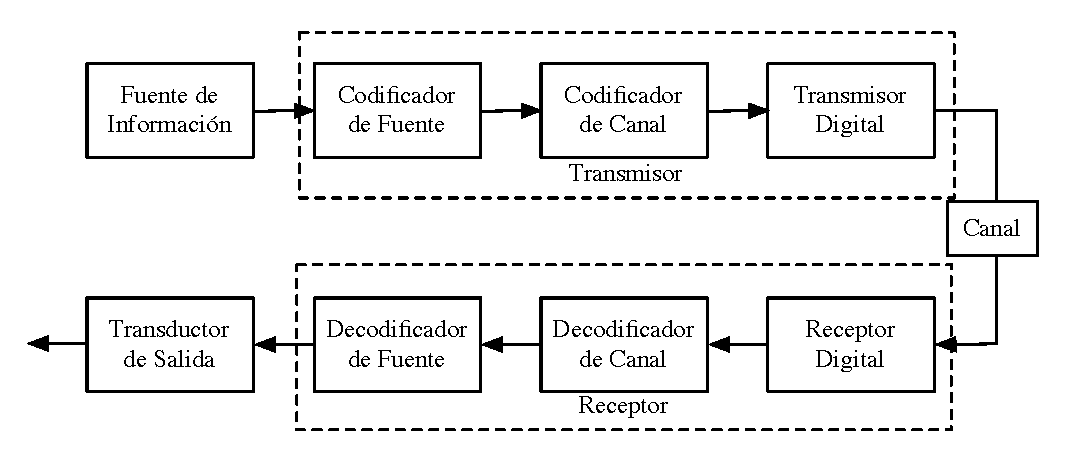
\includegraphics[width=0.95\linewidth]
{introduccion/figuras/fig01-01.pdf}
\caption{Modelo de un sistema de Comunicación Digital I}
\label{fig01-01}
\end{figure}
\end{lstlisting}
%\end{micuadro}

Y el resultado se muestra en la


Para incluir una tabla utilizamos las instrucciones siguientes:
%\nopagebreak 
\begin{lstlisting}[language=,caption={Inclusión de una tabla}, breaklines=true, label=prg01-02]
\begin{table}[htbp]
	\ttabbox
	{\caption{Tipos de transmisión y frecuencia central} 
	\label{tab2_1}}
		{
		\begin{tabular}{c c}
		\hline
		\rule[-8pt]{0pt}{22pt}{\bfseries{Tipo de Transmisión}}&
		 {\bfseries{Frecuencia central de transmisión}} \\
		\hline
		\rule{0pt}{14pt}Modem & 100-1800 Hz \\
		Radio AM & 530-1600 kHz \\
		Radio FM & 88-108 MHz \\
		Televisión & 178-216 MHz \\
		Telefonía móvil & 850 MHz-1,8 GHz \\
		Redes inalámbricas &  $2,4$ GHz \\
		Fibra óptica & $2\cdot 10^{14}$ Hz \\
		\hline
		\end{tabular}
		}
\end{table}
\end{lstlisting}

Y el resultado se muestra en la \autoref{tab2-1}.

\begin{table}[htbp]
	\ttabbox
	{\caption{Tipos de transmisión y frecuencia central} \label{tab2-1}}
		{
		\begin{tabular}{c c}
		\hline
		\rule[-8pt]{0pt}{22pt}{\bfseries{Tipo de Transmisión}}& {\bfseries{Frecuencia central de transmisión}} \\
		\hline
		\rule{0pt}{14pt}Modem & 100-1800 Hz \\
		Radio AM & 530-1600 kHz \\
		Radio FM & 88-108 MHz \\
		Televisión & 178-216 MHz \\
		Telefonía móvil & 850 MHz-$1,8$ GHz \\
		Redes inalámbricas &  $2,4$ GHz \\
		Fibra óptica & $2\cdot 10^{14}$ Hz \\
		\hline
		\end{tabular}
		}
\end{table}

Observemos  que en la parte inferior de las figuras y en la superior de las tablas (esta ha sido nuestra elección), se colocan textos explicativos sobre las mismas. El formato de este texto se logra mediante una sentencia facilitada por el paquete que se carga mediante el comando \comandos{usepackage}{caption}. El resto de paquetes utilizados realizan diversas tareas como, por ejemplo, \comandos{usepackage}{longtable}, que permite que una tabla se extienda a través de más de una página.

\subsection{Hiperenlaces}
Un primer paso a la hora de crear un documento es generar una versión en formato electrónico del mismo. Hemos decidido que ese formato sea \ttcolor{pdf} . En un formato pdf existe la posibilidad de crear hiperenlaces que facilitan la navegación a lo largo del mismo. Por ejemplo, el índice en un libro en formato pdf se generará, con la propuesta que hemos realizado, creando enlaces a las diversas partes del mismo. O bien, cuando nos referimos a una figura o tabla, es muy útil la existencia de esos enlaces al lugar exacto en el que se encuentra la figura o tabla.  El paquete responsable de realizar todas estas tareas se denomina \ttcolor{hyperref} y las sentencias que siguen a su carga realizan diversas tareas que pueden consultarse en la extensa documentación que lo acompaña. Sobre la línea 110 de \ttcolor{libroTipoETSI.tex} encontrará que puede modificar el color del enlace, puesto a negro por defecto.
% Por ejemplo, no habrá que olvidarse sustituir el literal \ttcolor{F. Javier Payán Somet y Juan José Murillo Fuentes} por el nombre del autor correspondiente.

\subsection{Tabla de contenido}
La generación de la tabla (o tablas) de contenido de un texto suficientemente largo suele ser una tarea sumamente laboriosa. \LaTeX\ facilita enormemente este trabajo mediante un conjunto de paquetes y comandos que se agrupan bajo el apartado genérico denominado TOC (Table Of Contents). En otra sección de este capítulo explicaremos cómo y dónde se incorporará esta tabla de contenidos. En este apartado nos centramos en explicar algunos aspectos de cómo se construye la principal tabla de contenidos, que denominamos  \ttcolor{Índice}.

Nuestra primera decisión fue establecer que en el índice deben aparecer hasta los apartados que hemos denominados \ttcolor{subsubsecciones}, lo que se logra mediante el \ttcolor{\{3\}} del comando \comandos{setcounter}{tocdepth} en \ttcolor{libroETSI.sty}. El formato de cada uno de los apartados se logra con el conjunto de sentencias que siguen y tienen una estructura bastante autoexplicativa. También hemos propuesto que no aparezcan los habituales puntos que existen entre el texto y el número de página correspondiente de muchos índices, ajustando a \ttcolor{10000} el parámetro \ttcolor{\textbackslash@dotsep}. 

Nuestra siguiente decisión afecta a la manera en la que hemos querido que aparezcan en el índice los índices del texto, valga la redundancia. No es trivial pero, básicamente, hemos definido dos listas, una para los elementos que aparecen antes del Índice General y otra para los  que aparecen después, al fina del texto, que se corresponden aproximadamente a lo que hemos denominado \ttcolorc{frontmatter} y \ttcolorc{backmatter}, respectivamente. Si no se desea cualquier índice, basta con comentar la línea correspondiente.

\subsection{Formatos de títulos, páginas y cabeceras y pies de páginas}
El aspecto de un libro está básicamente definido por el formato que se ha elegido para los diferentes títulos de las partes que lo constituyen, el formato de las páginas y qué queremos que aparezca en las cabeceras y pies de páginas del mismo. Todo esto se ha conseguido utilizando un paquete desarrollado por el español Bezos denominado \ttcolor{titlesec}, que se carga en nuestro fichero mediante la instrucción \comandos{usepackage[noindentafter, pagestyles,...]}{titlesec}.

El paquete nos permite definir los distintos tipos de páginas, de acuerdo con las instrucciones que se proporcionan en el mismo. Por ejemplo, con \comandos{newpagestyle}{esitscCD} creamos la página habitual en la mayor parte del texto, formada por el número en la parte exterior de la misma, en las páginas pares el nombre del capítulo en el que estamos y en las impares el nombre de la sección. Estos elementos se colocan encima de una raya horizontal que se ha definido previamente, tanto en su grosor como en su longitud.

Una vez definidos las diferentes tipos de páginas podemos definir, por ejemplo, que nuestra página por defecto será \ttcolor{esitscCD}, con la instrucción \comandos{pagestyle}{esitscCD}. Si queremos que una página determinada en un punto concreto sea diferente, si suponemos que, por ejemplo, el estilo de página \ttcolor{otroestilo} ha sido definido, basta situar la instrucción \comandos{thispagestyle}{otroestilo} en el punto deseado. Un ejemplo podemos encontrarlo en la manera que logramos que los capítulos empiecen siempre en páginas impares. Con ese fin, se utiliza el estilo de página \ttcolor{empty} en caso de que sea necesario.

Por último, el paquete \ttcolor{titlesec} nos permite definir cómo queremos que sean los titulares que usaremos en nuestros textos. Así,  la instrucción \comandos{titleformat}{\textbackslash section ...} establece que nuestras secciones estarán numeradas al nivel de capítulo, con el número de la sección fuera de margen \ttcolor{hang}, y con unas determinadas separaciones del texto, establecidas a través del comando \ttcolorc{titlespacing}. 

En todo caso, estos parámetros no se deberían de tocar, salvo en contadas ocasiones, y por ello se incluyen aquí estos detalles.

\subsection{Teoremas, propiedades, definiciones y demás}
En la escritura de cualquier texto científico los Teoremas, propiedades y demás elementos constituyen una parte muy significativa. Existen, de nuevo, múltiples posibilidades de tratar estos elementos, pero hemos considerado que las facilidades que suministra el paquete \ttcolor{ntheorem}, cargado mediante la instrucción \comandos{usepackage [thmmarks, amsmath, noconfig, hyperref, framed]}{ntheorem} se adapta perfectamente a nuestros gustos y decisiones. Por ejemplo, con el conjunto de instrucciones que se muestran en  el Código \ref{prg01-03}:

\begin{lstlisting}[language=TeX,caption={Teoremas, Lemas,...}, breaklines=true, label=prg01-03]
\theoremnumbering{arabic}
\theoremheaderfont{\aheadteoremas}
\theoremseparator{\hspace{.2em}}
\theorembodyfont{\itshape}
\newtheorem{teor}{Teorema}[section]
\newtheorem{lema}{Lema}[section]
\newtheorem{prop}{Propiedad}[section]
\newtheorem{coro}{Corolario}[teor]
\end{lstlisting}

\noindent hemos definido los Teoremas, Lemas, Propiedades y Corolarios. Centrándonos en los teoremas, las instrucciones anteriores definen que los teoremas estarán referenciados mediante un número \ttcolor{arabic}, con una numeración que será creciente desde la unidad dentro de cada sección de un determinado capítulo, \comandos{newtheorem\{teor\}}{Teorema}\ttcolor{[section]}. La fuente que se utilizará para que aparezca la palabra ``Teorema'' está definida por el comando \ttcolor{\textbackslash theoremheaderfont\{\textbackslash aheadteoremas\}}, el enunciado del teorema se realizará en itálica y para enunciar un teorema y su demostración utilizamos las siguiente instrucciones:

\begin{lstlisting}[language=TeX,caption={Teorema y Demostración}, breaklines=true, label=prg01-04]
\begin{teor}[Teorema de Pitágoras]
En un triángulo rectángulo...
\end{teor}
\begin{proof}
Sea el triángulo ABC...
\end{proof}
\end{lstlisting}

El resultado sería el siguiente:
\begin{teor}[Teorema de Pitágoras]
En un triángulo rectángulo...
\end{teor}
\begin{proof}
Sea el triángulo ABC...
\end{proof}

Podemos observar que al finalizar la demostración hemos incluido el símbolo $\blacksquare$. De manera análoga, están definidas las restantes entidades, incluyendo el comando que nos permite escribir los cuadros de elementos de la programación.

\subsection{Índices de palabras y glosarios}
Con los paquetes index y glossaries podemos incluir índices de palabras y listas con definiciones, ya sea de acrónimos u de otro tipo. Por ejemplo, se podría usar también para definir magnitudes o la notación utilizada.
 
%http://en.wikibooks.org/wiki/LaTeX/Indexing
\subsubsection{Índices de palabras}
\index{Indice de palabras@Índice de palabras!index}%\index{\'Indice de palabras!index}\index{Índice de palabras!indexit}
Para construir un índice de palabras\index{Indice de palabras@Índice de palabras}, como el que puede encontrar al final de este texto, se incluye el paquete \comandos{usepackage}{imakeidx} con algunas opciones. Para incluir una palabra  en el índice utilizamos   \comandos{index}{palabra} justo detrás de la palabra que queramos indexar. Si queremos agrupar en un grupo diferentes subpalabras \index{Indice de palabras@Índice de palabras!subpalabra}, utilizamos \comandos{index}{palabra!subpalabra}. Es importante no olvidar ejecutar \ttcolor{makeindex}, al igual que ejecuta latex o bibtex para componer el texto o generar la bibliografía. Otro detalle importante es poner los índices con mayúsculas o con minúsculas, pero todos iguales. De esta forma, cuando se genere el índice de palabras no queden algunas con la primera letra en mayúsculas y otras no. Por último, con las instrucciones de compilación que se detallan un poco más adelante, las palabras en español que empiecen por tilde se indexan al final. Para evitarlo, y que aparezcan en su sitio, tiene que escribir primero la palabra sin tilde seguida de arroba y la palabra con tilde, como por ejemplo \ttcolorc{index\{Indice de palabras@Índice de palabras\}}. 

\subsubsection{Glosario}
Un glosario con acrónimos u otros términos se realiza en este texto utilizando\\
 \comandos{usepackage [acronym]}{ glossaries}. 
 Para definir un acrónimo, basta con incluir antes del comienzo del documento una línea del tipo:\\
 \comandos{newacronym[type=main]\{etiqueta\}\{acrónimo\}}{nombre completo}, 
 \\
 como por ejemplo\\
 \comandos{newacronym[type=main]\{ETSI\}\{ETSI\}}{Escuela Técnica Superior de \\Ingeniería}. 
 \\
 En esta orden el primer argumento es el identificador o etiqueta, el segundo es el acrónimo o abreviatura y el tercero es el nombre completo al que hace referencia el acrónimo o abreviatura. Para utilizar luego la abreviatura o acrónimo, y se pueda luego generar un índice que indique en qué página se ha usado, se utiliza \comandos{gls}{etiqueta}. 

\subsubsection{Compilación de índices de palabras y glosarios}
Existen distintos comandos para generar el índice y el glosario. Puede utilizar los que estime oportunos. Aquí se ofrece una solución para realizarlo.

El comando más usado es \ttcolor{makeindex}. Habría que llamar dos veces a este comando, con distintos argumentos, si se incluye el glosario además del índice. En Macintosh si utiliza el comando \ttcolor{lualatexmk}, uno de los engines de TeXShop\index{engine}, el índice de palabra y el glosario se generarán de forma automática. 
%Puede usar Texindy\index{Texindy} para una presentación del índice de palabras con otra presentación.

En Windows, tendrá que ejecutar PDFLatTeX ó LatexMk, luego tendrá que ejecutar makeindex tal cual para generar el índice de palabras. Para generar el glosario tendrá que definir un comando de usuario, tal como sigue. Vaya al menú `Usuario', en texmaker, y allí a `Comandos de Usuario' y dentro de este a `Editar Comandos de Usuario'. En cualquiera de los comandos defina uno nuevo con el título que quiera, por ejemplo glosario, y en el campo comando, incluya la siguiente línea\footnote{Si usase el texmaker en Mac-OS tendría que pulsar el asistente para seleccionar makeindex. Aparecería en el campo comando algo así como \ttcolor{''makeindex'' \%.idx}, donde el asistente habrá encontrado la carpeta donde está el comando makeindex. Sustituya el final, \%idx, por  -s \%.ist -t \%.glg -o \%.gls \%.glo, de forma que el campo comando quede como sigue:
 \ttcolor{''/usr/texbin/makeindex'' -s \%.ist -t \%.glg -o \%.gls \%.glo}}

Una vez definido este comando de usuario, ejecútelo, y vuelva a ejecutar PDFLaTeX o LatexMk.

\section{Antes del documento}
Antes de empezar la edición del documento, además de cargar los ficheros de estilos \ttcolor{LibroETSI.sty} y \ttcolor{edicionLibro.sty} (o el correspondiente al documento),  hemos creído necesario realizar una serie de operaciones que faciliten nuestro trabajo o lo configuren de una determinada manera. %Además, hay que incluir la portada.

\subsection{Fichero de notación: notacion.sty}
Hemos considerado interesante incluir un fichero de notaciones que son de amplia utilidad dentro del área de conocimiento de los autores. Su uso es completamente opcional pero se ha utilizado ampliamente en la elaboración de este texto. Simplifica enormemente la escritura hacer uso de ficheros de este tipo y prácticamente cada autor utiliza el suyo propio.

Como ocurría con el fichero \ttcolor{LibroETSI.sty}, es necesario que se cargue, incluyendo la instrucción \comandos{usepackage}{notacion} al comienzo del fichero principal. Puesto que su uso resulta evidente, no hemos considerado necesario realizar una documentación precisa sobre el mismo más allá de los propios comentarios que acompañan las definiciones del fichero, y que el lector puede consultar abriéndolo. Nótese que existe además una carpeta con este nombre. En esta carpeta se ha incluido un ejemplo de notación que podría ponerse al comienzo de un documento. Sobre este documento, se puede añadir o quitar lo que se desee.

\subsection{Fuente del texto}
Las instrucciones incluidas en el código \ref{prg01-05} y que pertenecen al fichero \ttcolor{LibroETSI.sty} 
 se pueden modificar para cambiar la fuente del texto.  En primer lugar, debemos actuar de forma diferente si queremos utilizar la fuente Minion Pro o no.  Si hemos definido como \ttcolor{true} el parámetro correspondiente, en el caso que estemos compilando con \LaTeX\ no debemos hacer nada. Sin embargo, en el caso de utilizar \LuaLaTeX\ debemos declarar que la fuente va a ser Minion Pro y modificar ligeramente su tamaño.
 
Si no vamos a utilizar una fuente Minion Pro, en el caso de \LuaLaTeX\ se puede utilizar para el texto cualquier fuente OTF o TTF que el usuario posea de forma legal, y se encuentre instalada, lo que depende del sistema operativo (SO) utilizado. En nuestro caso, observad que hemos utilizado una fuente Time New Roman  pues suele estar instalada en la mayoría de los SO. Se proponen asimismo un par de alternativas si prefiere otras fuentes.
 
El código incluido detecta si se no se está utilizando \LuaLaTeX\, en cuyo caso se usa una fuente equivalente a una Times, cargada mediante el comando estándar \comandos{usepackage}{tgtermes}. Hay otras opciones comentadas, y se pueden buscar otras fuentes. 
 
\begin{lstlisting}[language=,caption={Fuente del texto}, breaklines=true, label=prg01-05]
%:Para modificar fácilmente la fuente del texto. 
\makeatletter
\ifdtsc@Minion % Queremos utilizar la fuente Minion y lo hemos declarado al principio
	\ifluatex
		\setmainfont[Renderer=Basic, Ligatures=TeX,	% Fuente del texto 
		Scale=1.01,
		]{Minion Pro}
   		% En este caso conviene modificar ligeramente el tamaño de las fuentes matemáticas
		\DeclareMathSizes{10}{10.5}{7.35}{5.25}
		\DeclareMathSizes{10.95}{11.55}{8.08}{5.77}
		\DeclareMathSizes{12}{12.6}{8.82}{6.3}
	\fi
\else
	\ifluatex
		% Para utilizar la fuente Times New Roman, o alguna otra que se tenga instalada
		\setmainfont[Renderer=Basic, Ligatures=TeX,	% Fuente del texto 
		Scale=1.0,
		]{Times New Roman}
%		\setmainfont[Renderer=Basic, Ligatures=TeX,	% Fuente del texto 
%		]{Adobe Garamond Pro}
%		\setmainfont[Renderer=Basic, Ligatures=TeX,	% Fuente del texto 
%		]{Palatino LT Std}
	\else
		\usepackage{tgtermes} 	%clone of Times
		%\usepackage[default]{droidserif}
		%\usepackage{anttor} 	
	\fi
\fi
\makeatother
\end{lstlisting}

Si se intenta utilizar una fuente que no está instalada (dentro del sistema operativo) la compilación con \LuaLaTeX\ daría error. Si se instala una nueva fuente y se desea utilizar, se puede tratar de modificar las líneas de código que se suministran como ejemplo. La primera vez que se utilice esa nueva fuente, \LuaLaTeX\ tardará algo más en compilar pues necesita generar una serie de ficheros internos.

La principal ventaja en el uso de \LuaLaTeX\ la encontramos en la facilidad para utilizar diferentes fuentes en diferentes lugares y con diferentes características (tamaño, color, etc) muy fácilmente configurables. Puede ser interesante leer el fichero \ttcolor{fontspec.pdf} para conocer cómo se realizan estos cambios. 

En caso de utilizar el motor pdfLatex, la elección más sencilla se realiza como hemos dicho mediante paquetes específicos tales como \comandos{usepackage}{tgtermes}. Puede consultarse la dirección \url{http://www.tug.dk/FontCatalogue/alphfonts.html} para conocer las posibilidades más habituales. 

Por último: como ya hemos dicho, todo lo anterior únicamente afecta a la elección de las fuentes del texto. La elección de las fuentes matemáticas (texto dentro de matemática, símbolos, letras griegas, etc) se controla de manera completamente diferente mediante paquetes específicos. En el \autoref{estilo} volveremos sobre este asunto. En concreto, observar que en el caso de compilar con la opción \ttcolor{Minion=true} y existir el fichero de estilo \ttcolor{MinionPro.sty} (no confundir con la fuente Minion Pro; si no existiera el fichero, aparecería un error), se propone el uso de la fuente Minion Pro como fuente matemática, junto con los símbolos de la fuente MnSymbol. En caso contrario, se hará uso de una fuente Times (en realidad, de una extensión de la misma). 

No todas las fuentes pueden usarse como fuentes matemáticas y en la dirección \url{http://www.tug.dk/FontCatalogue/alphfonts.html} se encuentran recogidas las que si tienen soporte matemático. Es importante señalar además que no todas las combinaciones de fuente de texto y fuente matemática son tipográficamente adecuadas. 

\subsection{Cubierta y primeras páginas}
Se ha diseñado esta plantilla para que tome una imagen de fondo y a partir de ésta se incluyan los datos de título, autor, etc, para generar la portada del documento. La portada propuesta es distinta para proyectos fin de carrera y similares que para libros o tesis. Todo esto se ha hecho diseñando una serie de funciones que las generan, tomando los datos que se definen en la cabecera del fichero principal. Así, en el \ttcolor{libroTipoETSI.tex}, se puede definir el título de la obra, el autor, etc. En el caso de \ttcolor{pfcTipoETSI.tex} y \ttcolor{tesisTipoETSI.tex}, se puede definir además el director, el tipo de proyecto (máster, grado y carrera), y otros parámetros. Las imágenes de fondo de la cubierta también se llaman desde este fichero, así como la imagen al pié de la hoja interior con el título y autor de la obra (para libros). La imagen central de la cubierta está en la carpeta figuras, con nombre \ttcolor{imagenLibro.png}. Puede incluir la imagen deseada en esta carpeta salvándola con este mismo nombre. Preste atención a que el formato es rectangular. Para introducir la imagen del logo del departamento en el proyecto fin de carrera/grado/máster, puede retocar la imagen de fondo, cortando el logo existente e insertando el deseado. Estas imágenes están en la carpeta figuras. 

Para cambiar cualquier otro aspecto, tales como el tamaño de la figura de la cubierta ó los créditos de la cubierta, tendrá que modificar el fichero \ttcolor{edicionLibro.sty} en este caso de un libro. 

%En el ejemplo que se presenta para libros, el latex toma una imagen de fondo, y otra, imagenLibro.png,  de la portada para incluir además de los datos de título y autores, definidos al comienzo del fichero \ttcolor{portadaLibro.tex}, una imagen superpuesta representativa de la temática del texto. Los autores pueden cambiar esta imagen fácilmente por otra acorde a su texto.

%Sería interesante poner algo sobre citas

\endinput
